\documentclass[12pt, a4paper]{article}
\usepackage{cv_style}

\newcommand{\putname}{David Hilbert}

\lhead{\textcolor{light-gray}{\small\scshape{\putname}}}
\chead{\textcolor{light-gray}{\small\scshape{CV}}}
\rhead{\textcolor{light-gray}{\small\thepage}}


\begin{document}
\begin{longtable}{@{} p{0.29\textwidth} >{\RaggedRight}p{0.46\textwidth} >{\RaggedRight}p{0.22\textwidth}}
  \\
  & \textbf{\putname} 
  & \multirow{4}{*}{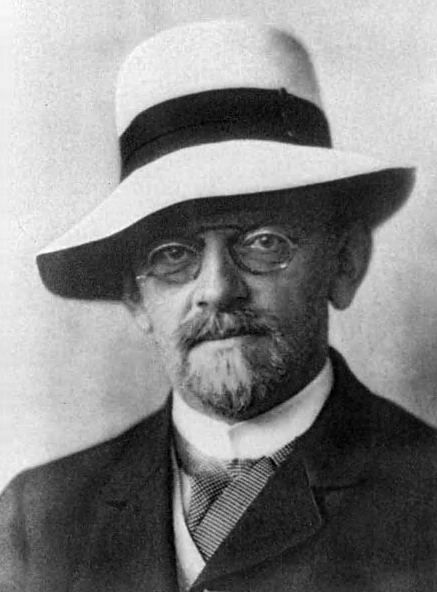
\includegraphics[width=3cm, height=3cm, keepaspectratio]{hilbert}} \\
  Address
  & Wilhelm-Weber-Straße 29 \\
  & 37075 G\"ottingen \\
  Email
  & \href{mailto:}{david.h@mail.com} \\
  GitHub
  & \href{https://github.com/linusroe}{linusroe} \\
\end{longtable}

\begin{longtable}{@{} p{0.29\textwidth} >{\RaggedRight}p{0.68\textwidth}}
  \textcolor{midblue}{\textbf{Occupation}}
  & \textbf{University of Göttingen} \\
  1886 - 1895
  & Professor \\
  & \\

  & \textbf{University of Königsberg} \\
  1886 - 1895
  & Lecturer \\
  & \\


  \textcolor{midblue}{\textbf{Higher Education}}
  & \textbf{University of Königsberg} \\
  1880 - 1885
  & PhD, Mathmatics  

  Thesis: ``Über invariante Eigenschaften spezieller
  binärer Formen, insbesondere der Kugelfunktionen''

  Advisor: Carl Louis Ferdinand von Lindemann \\
  & \\


  \textcolor{midblue}{\textbf{Early Education}}
  & \textbf{Wilhelms-Gymnasium, Königsberg} \\
  1879 - 1880
  & Abitur \\
  & \\

  & \textbf{Friedrichskollegium, Königsberg} \\
  1875 - 1879 
  & School \\
  & \\


  \textcolor{midblue}{\textbf{Scholarships}}
  & \textbf{Emmy Noether Programme} \\
  1885 - 1895
  & DFG \\
  & \\


  \textcolor{midblue}{\textbf{Languages}}
  & German (Mother tongue) \\
  & Language of Mathmatics (First Language) \\
  & \\


  \textcolor{midblue}{\textbf{Areas of interest}}
  & Axiomatization of geometry, Hilbert's 23 problems,
  Cue sports \\
  & \\

  \newpage

  \textcolor{midblue}{\textbf{References}}
  & \textbf{Billy Twillig} \\
  & Logicon Project \\
  & Field Experiment Number One \\
  & A distant Land \\
  Email
  & twillig@fen1.de \\
  & \\

\end{longtable}
\end{document}
